\section{Introduction}
In the present article, we replicate the results of Huisman \& Weissing 1999 \textit{Biodiversity of plankton by species oscillations and chaos} \cite{1999:Huisman}, an attempt to resolve the paradox of the plankton \cite{1961:Hutchinson} with a nonlinear ordinary differential equation model based on resource competition theory.\\

According to many mathematical models, the number of phytoplankton species in a single homogeneous medium cannot exceed the number of separate resources available \cite{1960:Hardin,1973:Phillips,1980:Armstrong}. However it is very common to observe more species than easily identifiable resources in field conditions. This led Hutchinson to formulate the paradox of the plankton \cite{1961:Hutchinson}. Using numerical simulations of their ODE model, Huisman \& Weissing \cite{1999:Huisman} showed that ``supersaturated coexistence'' is possible, where more consumer species than resource items coexist through oscillations or chaos. We attempt here to check this finding. \\

In addition to the replication of the numerical results of Huisman and Weissing \cite{1999:Huisman}, we also present two novel numerical experiments inspired by follow-up articles, \textit{Does ``supersaturated coexistence'' resolve the ``paradox of the plankton'' ?} by Schippers et al. 2001 \cite{2001:Schippers}, and \textit{Towards a solution of the plankton paradox: the importance of physiology and life history} by Huisman et al. 2001 \cite{2001:Huisman}. These articles suggested that supersaturated coexistence might be difficult to obtain outside of the restricted parameter scenarios considered in the original article. Schippers et al. \cite{2001:Schippers} assessed the sensitivity of diversity to parameter perturbations. They did so changing parameters for one species at a time, concluding that supersaturated coexistence was unlikely, while Huisman et al. \cite{2001:Huisman} showed how some trade-offs can make parameter combinations favourable to coexistence emerge (although most of the scenarios they consider confirm the results of Schippers et al. \cite{2001:Schippers}). Here, we further consider mild perturbations of intrinsic population growth rates of all species at once (though not necessarily in the same direction), a hypothesis which we deem coherent with whole-ecosystem perturbations. If supersaturated coexistence is a likely coexistence mechanism, small changes to population growth rates should not massively affect the number of coexisting species. 

\section{Model}

We describe below the model of phytoplankton community dynamics of Huisman \& Weissing \cite{1999:Huisman}. Let $N_i$ and $R_j$ respectively be the population density of species $i$ and concentration of resource $j$, $i\in[\![1,n]\!]$ and $j\in[\![1,k]\!]$ with $n$ and $k$ the number of different species and resources. The time derivatives of $N_i$ and $R_j$ are given by: \\

\begin{align}
	& \frac{dN_i}{dt}= N_i(\mu_i(R_1,...,R_k)~-~m_i)\\
	& \frac{dR_j}{dt}= D(S_j-R_j) - \sum_{i=1}^n c_{ji} 
\mu_i(R_1,...,R_k)N_i
\end{align}

with parameters

\begin{align*}
& m_i \text{ the mortality rate of species $i$}\\
& D \text{ the system's turnover rate}\\
& S_j \text{ the supply concentration of resource $j$}\\
& c_{ji} \text{ the content of resource $j$ in species $i$}\\
& \mu_i \text{ the growth rate of species $i$, defined using the Monod equation and Liebig's law of minimum: }
\end{align*}

\begin{align}
&\mu_i(R_1,...,R_k)~=~\min_{j\in[\![1,k]\!]} \left( \frac{r_iR_j}{K_{ji}+R_j} \right). 
\end{align}

The growth rates are defined using: 
\begin{align*}
&r_i \text{ the maximum growth rate of species $i$}\\
&K_{	ji} \text{ the half-saturation constant for resource $j$ of species $i$.}
\end{align*}

In order to reproduce the results of Huisman \& Weissing \cite{1999:Huisman}, the differential equations were integrated using the \texttt{deSolve} \cite{deSolve} package in its 1.32 version in \texttt{R} \cite{R} 4.2.0, using the same parameter sets as in the original article.\\

Multiple simulations are performed and illustrated in the original article as well as here: \\
In Figure \ref{figures:Fig1} a) and b), 3 species are competing for 3 resources, in c), 6 species are competing for 3 resources (supersaturation) and in d), 9 species are competing for 3 resources (supersaturation again). In Figure \ref{figures:Fig2}, 5 species are competing for 3 resources. In Figure \ref{figures:Fig3}, 5 species are competing for 5 resources. In Figure \ref{figures:Fig4}, 12 species are competing for 5 resources. In Figure \ref{figures:Fig2} and Figure \ref{figures:Fig1} a), b) and for the bifurcation diagram of Figure \ref{figures:Fig3}, all of the species are introduced at the same time in the simulation. In Figure \ref{figures:Fig4} and Figure \ref{figures:Fig1} c), d), the species were introduced sequentially. Huisman et al. \cite{1999:Huisman} have provided the starting times of each species introductions when needed, in addition to the parameters.\\


As Schippers et al. \cite{2001:Schippers}, we were wondering how and why the parameter sets were initially chosen, and if the results would remain the same for slightly different parameters. Several simulations were made in Schippers et al. paper \cite{2001:Schippers} and Huisman et al.'s response \cite{2001:Huisman}, in order to evaluate how robust was supersaturated coexistence. In the same spirit, we carried out new numerical experiments with a slightly different perspective.\\

We chose to focus on evaluating the robustness of the last simulation of Huisman \& Weissing \cite{1999:Huisman}, displayed on Figure \ref{figures:Fig4}. We focused on perturbating the growth rate parameter, $r_i$, denoted as $\mu_{\text{max}}$ in the follow-up articles \cite{2001:Schippers, 2001:Huisman}. As changing only a single one of the $n$ intrinsic growth rates $r_i$ (as done earlier in the follow-up articles \cite{2001:Schippers, 2001:Huisman}) appeared a little artificial to us, we chose to randomly perturb all of the $n~~r_i$ at once, as would typically do an ecosystem-wide perturbation that is not directly related to the modelled resources. Furthermore, it is overall more realistic, as some articles \cite{2015:Edwards} suport the idea that growth rates may vary between species even in the absence of perturbations. In a first numerical experiment, we considered the exact same invasion sequence as Huisman \& Weissing \cite{1999:Huisman}.  In a second step, we started with the full set of species at once.\\
\\
In order to conduct the numerical experiments proposed earlier, the method used to plot the fourth Figure has been reused. The two experiments were conducted 500 times each, with as many different parameter sets: the $r_i$, normally all set to the value of $1$, were drawn according to a truncated normal distribution. The mean was $\mu=1$ and the variance was $\sigma=0.1$, corresponding to CV=10\%. The distribution was truncated using $\mu\pm3\sigma$, in other words $r_i$ values remain between $0.7$ and $1.3$ (and most values are much closer to 1). This range of values remains consistent, and even conservative, when compared to experimental values \cite{2015:Edwards}, where CVs can be larger. As we are trying to challenge the robustness of the replicated simulation, we do not change any other parameters: thus we will only conduct the simulations for a duration of 10000 days, as the original simulations. However, in order to easily visualise how biodiversity changes over time, we also measure the number of different species at the times used in the article to introduce new species, i.e. after 1,000, 3,000 and 5,000 days.\\~\\ 

\section{Results}

\subsection{Reproduction}

We were able to replicate the four figures of Huisman \& Weissing \cite{1999:Huisman}, presented below. 

\begin{figure}[H]
\begin{center} 
 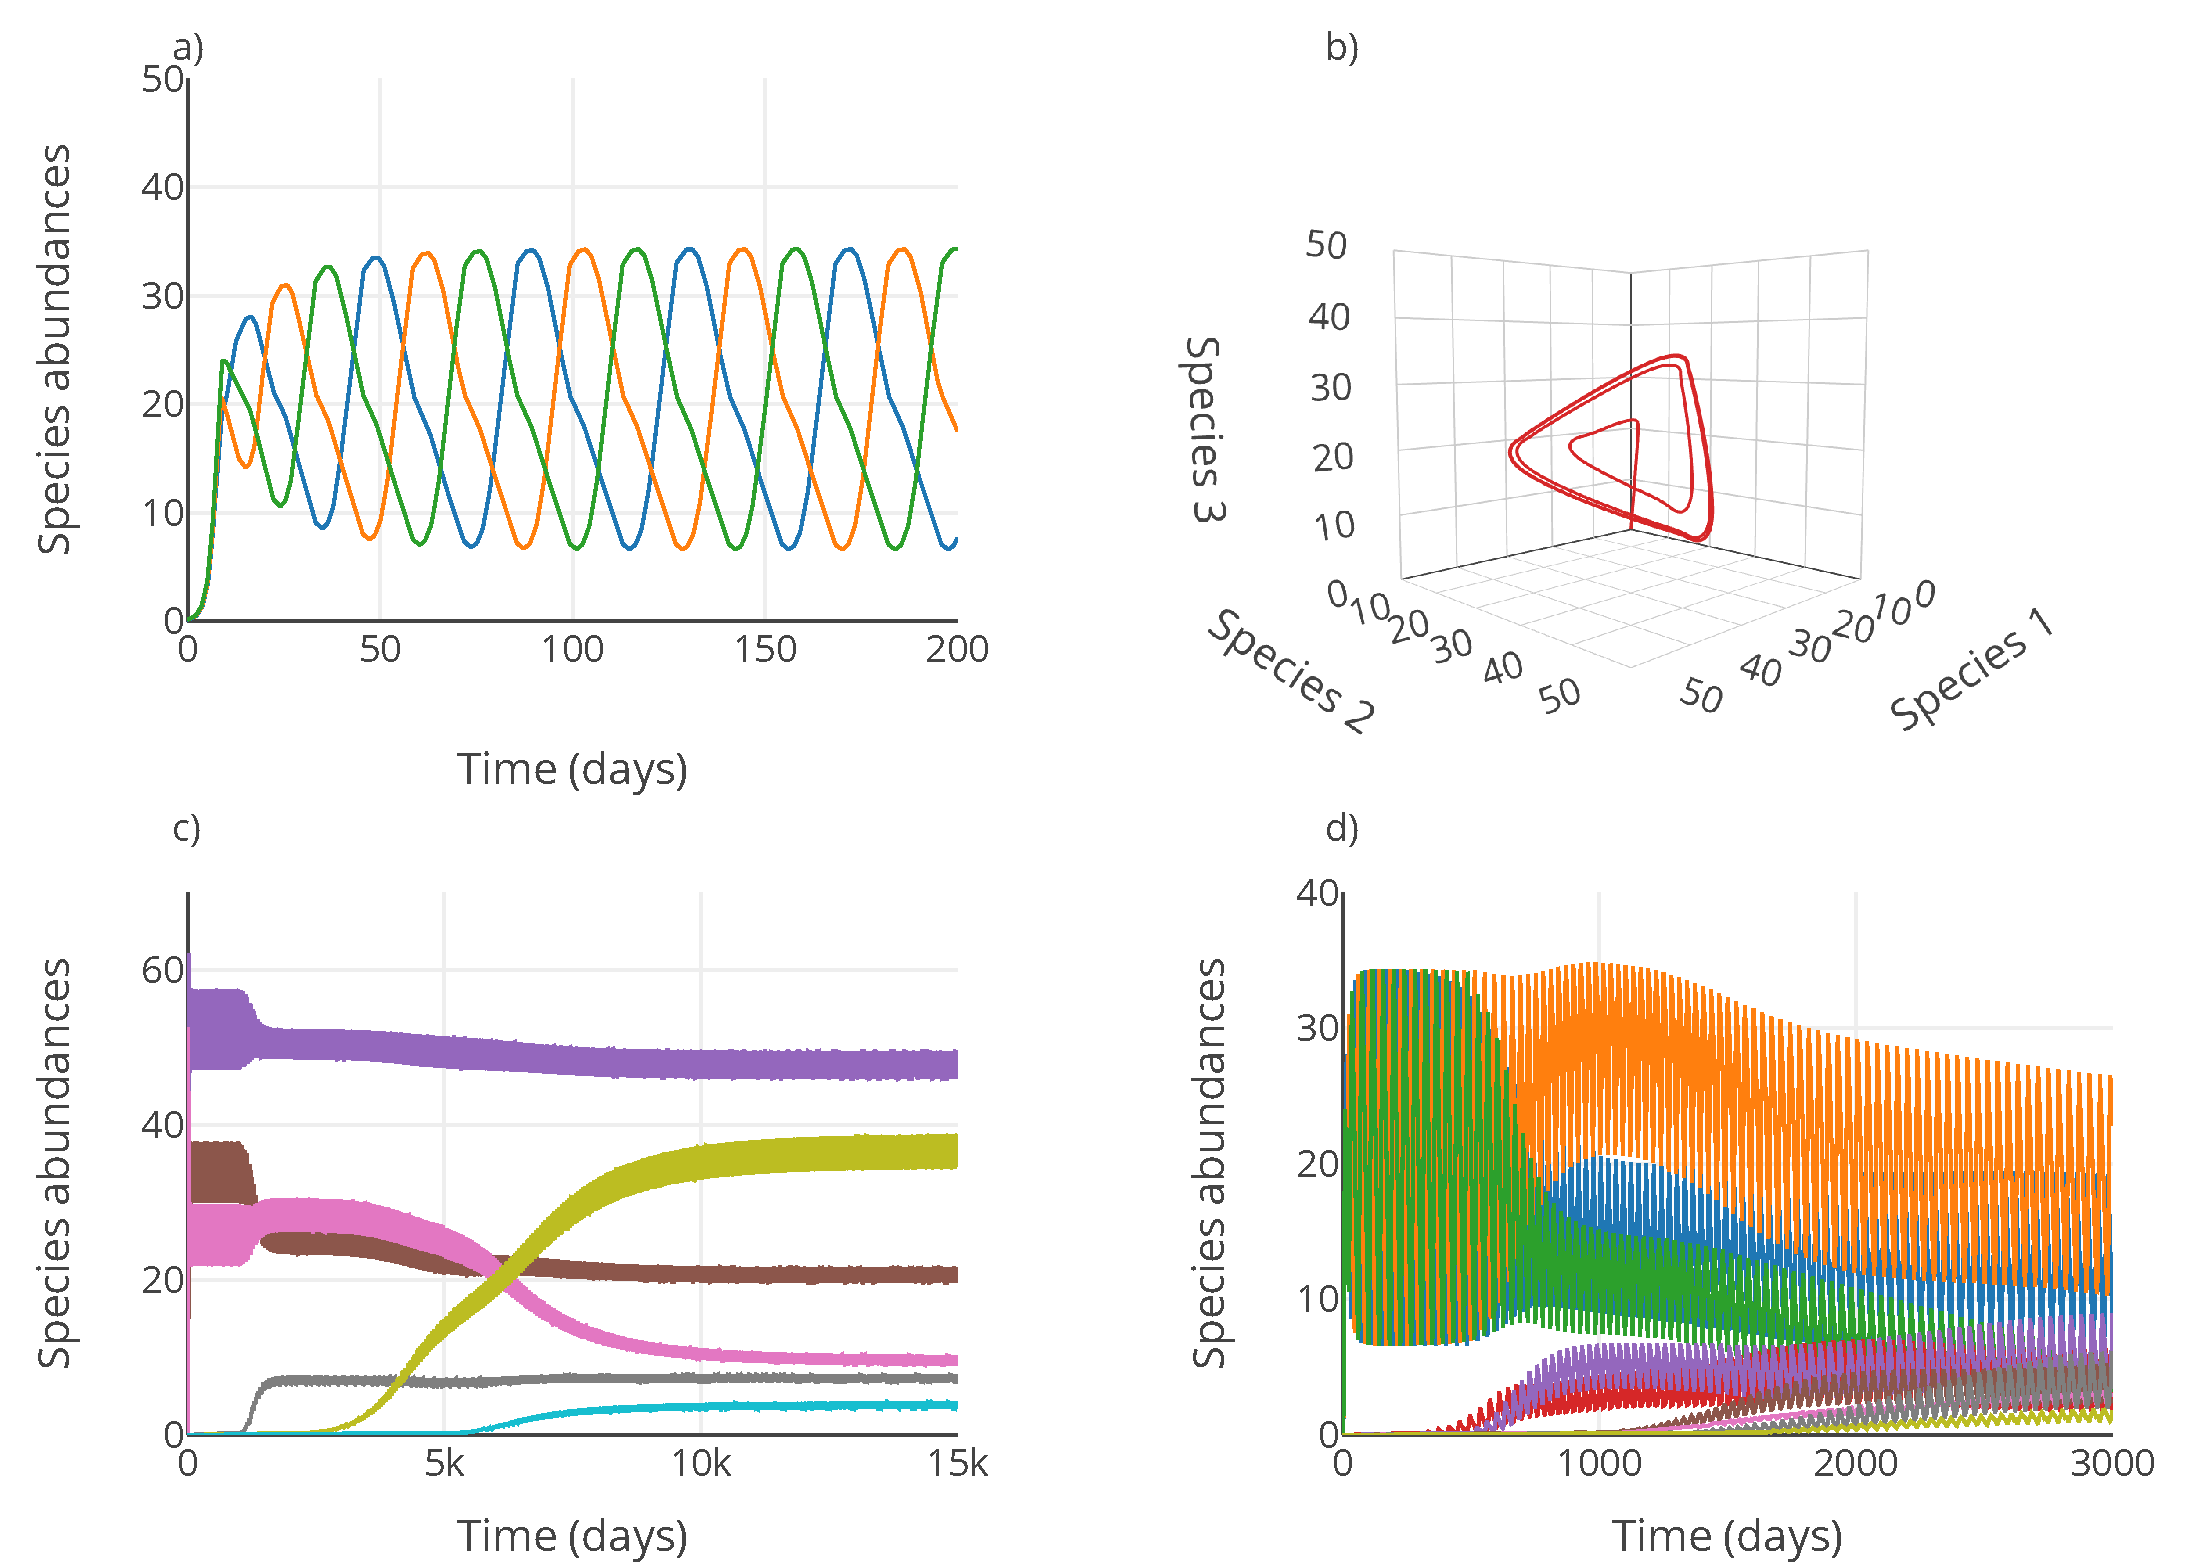
\includegraphics[width=1\textwidth]{../Code/Figures/Figure_1.pdf}
  \caption{Oscillations on three resources. a), Time course of the abundances of three species competing for three resources. b), The corresponding limit cycle. c), Small-amplitude oscillations of six species on three resources. d), Large-amplitude oscillations of nine species on three resources.}
  \label{figures:Fig1}
\end{center}
\end{figure}

\begin{figure}[H]
\begin{center} 
 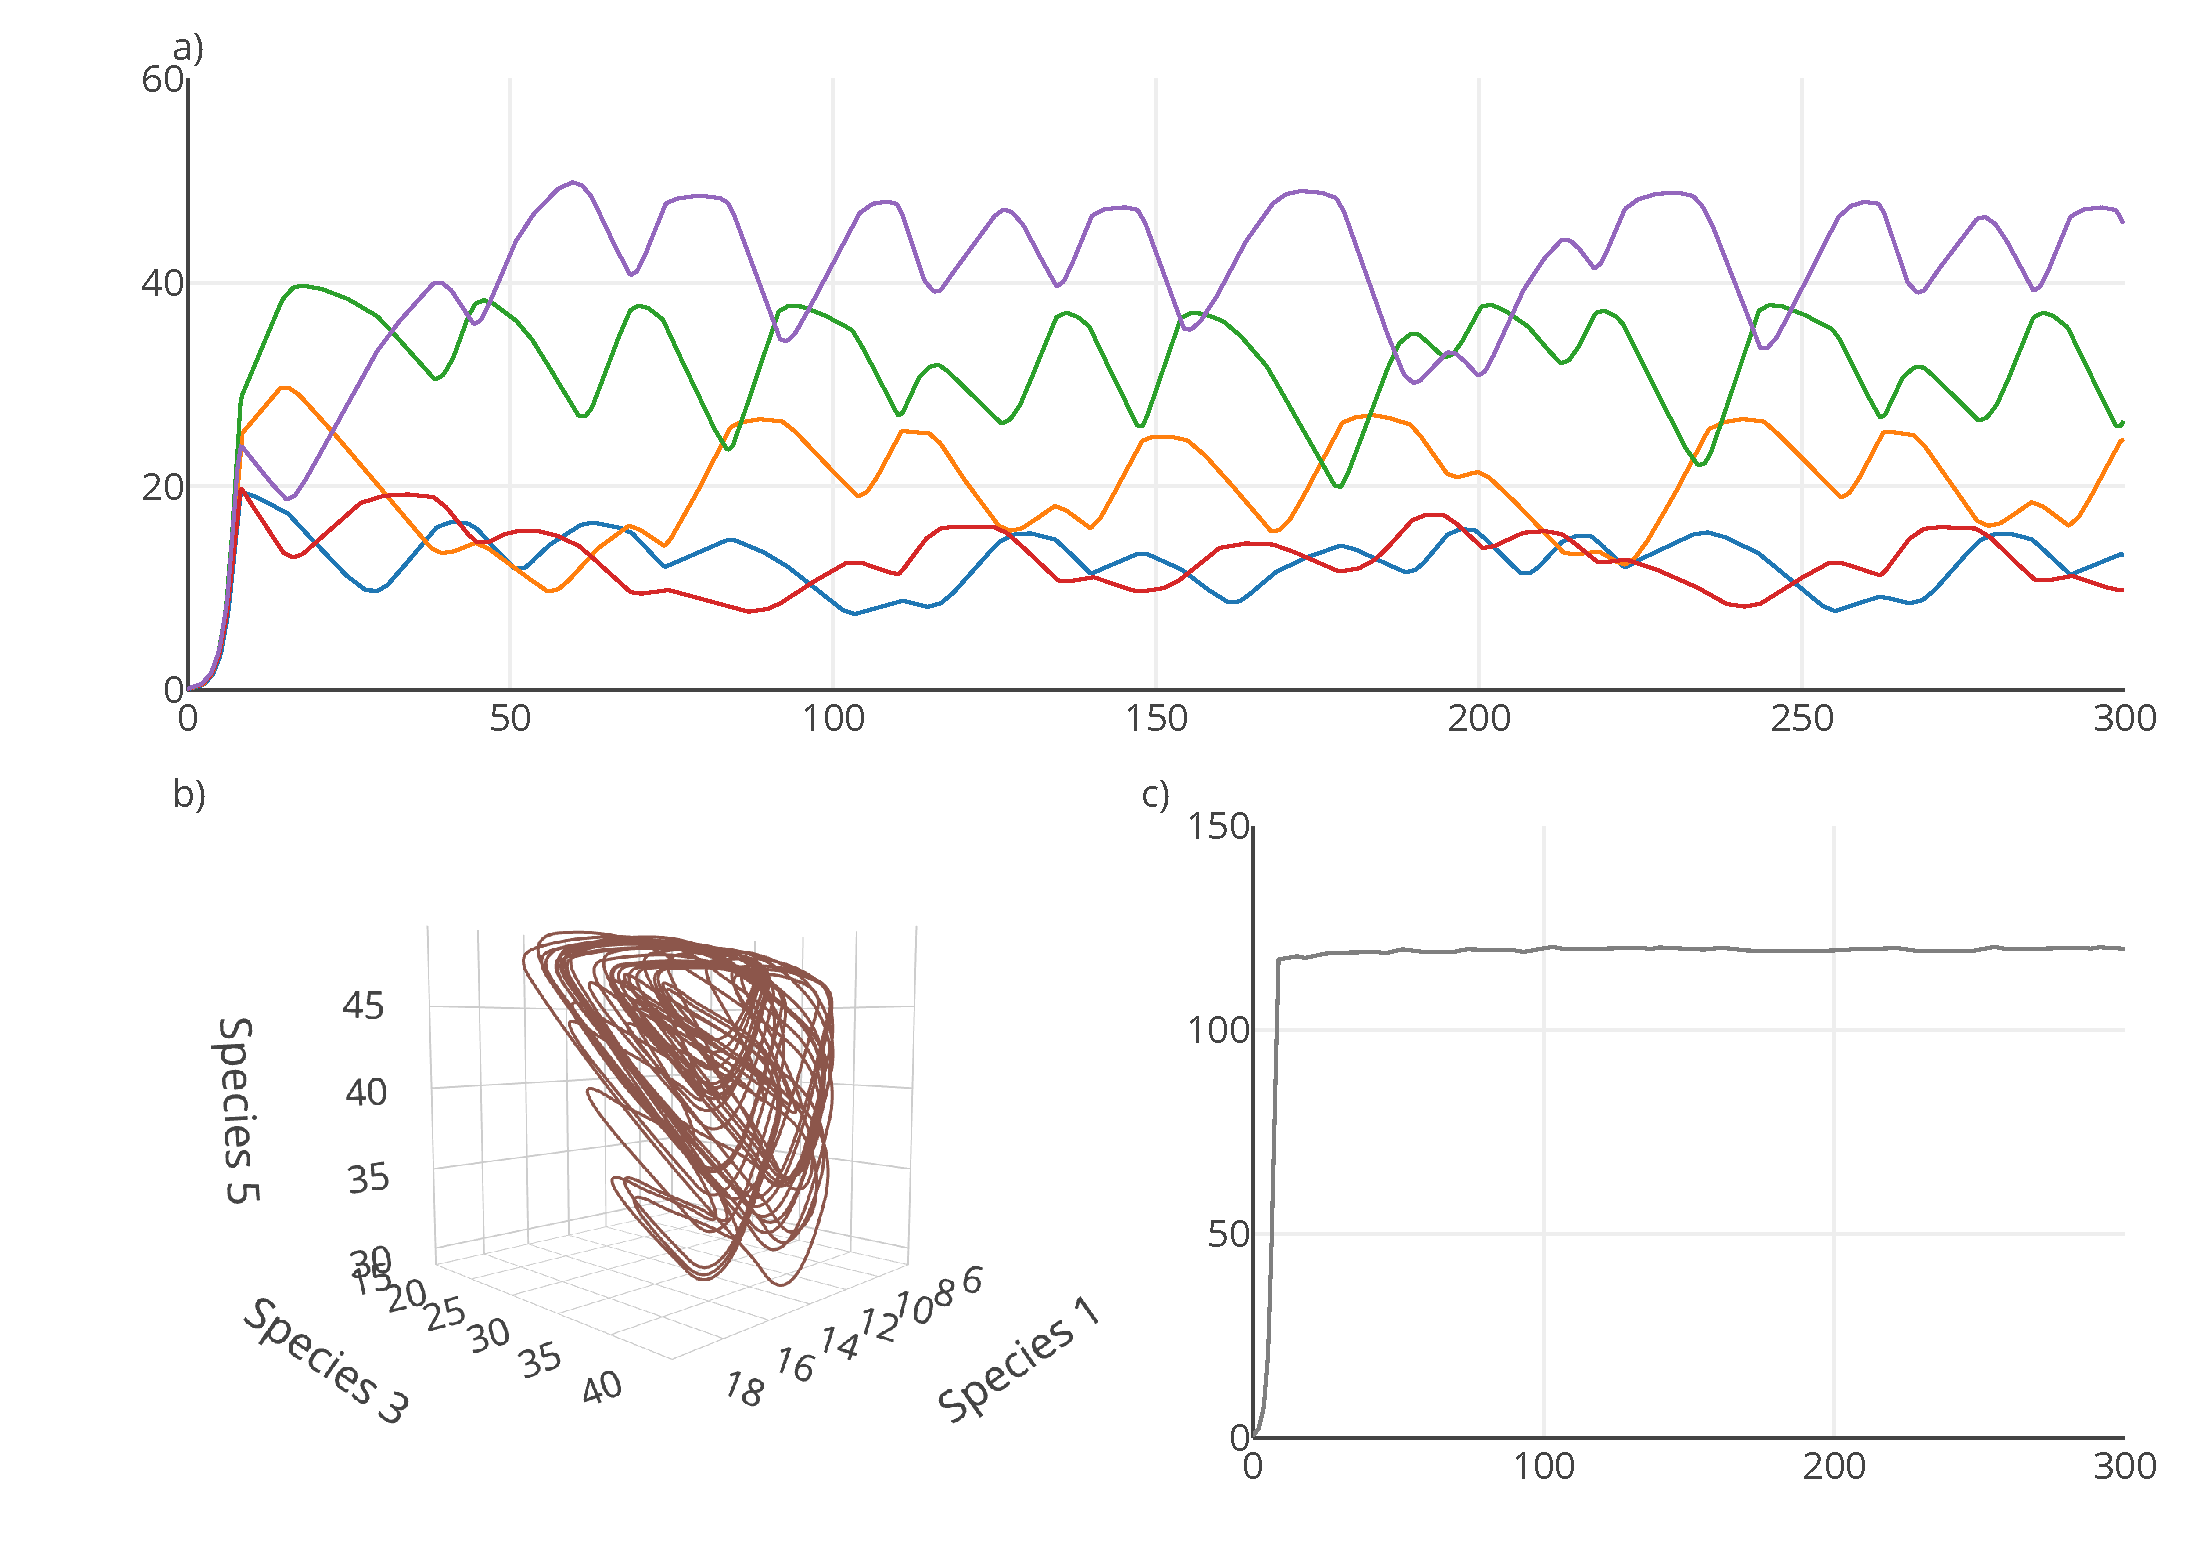
\includegraphics[width=1\textwidth]{../Code/Figures/Figure_2.pdf}
  \caption{Chaos on five resources. a) Time course of the abundances of five species competing for five resources, b) The corresponding chaotic attractor. The trajectory is plotted for three of the five species, from the period from $t= 1,000$ to $t=2,000$ days, c) Time course of total community biomass.}
  \label{figures:Fig2}
\end{center}
\end{figure}

\begin{figure}[H]
\begin{center} 
 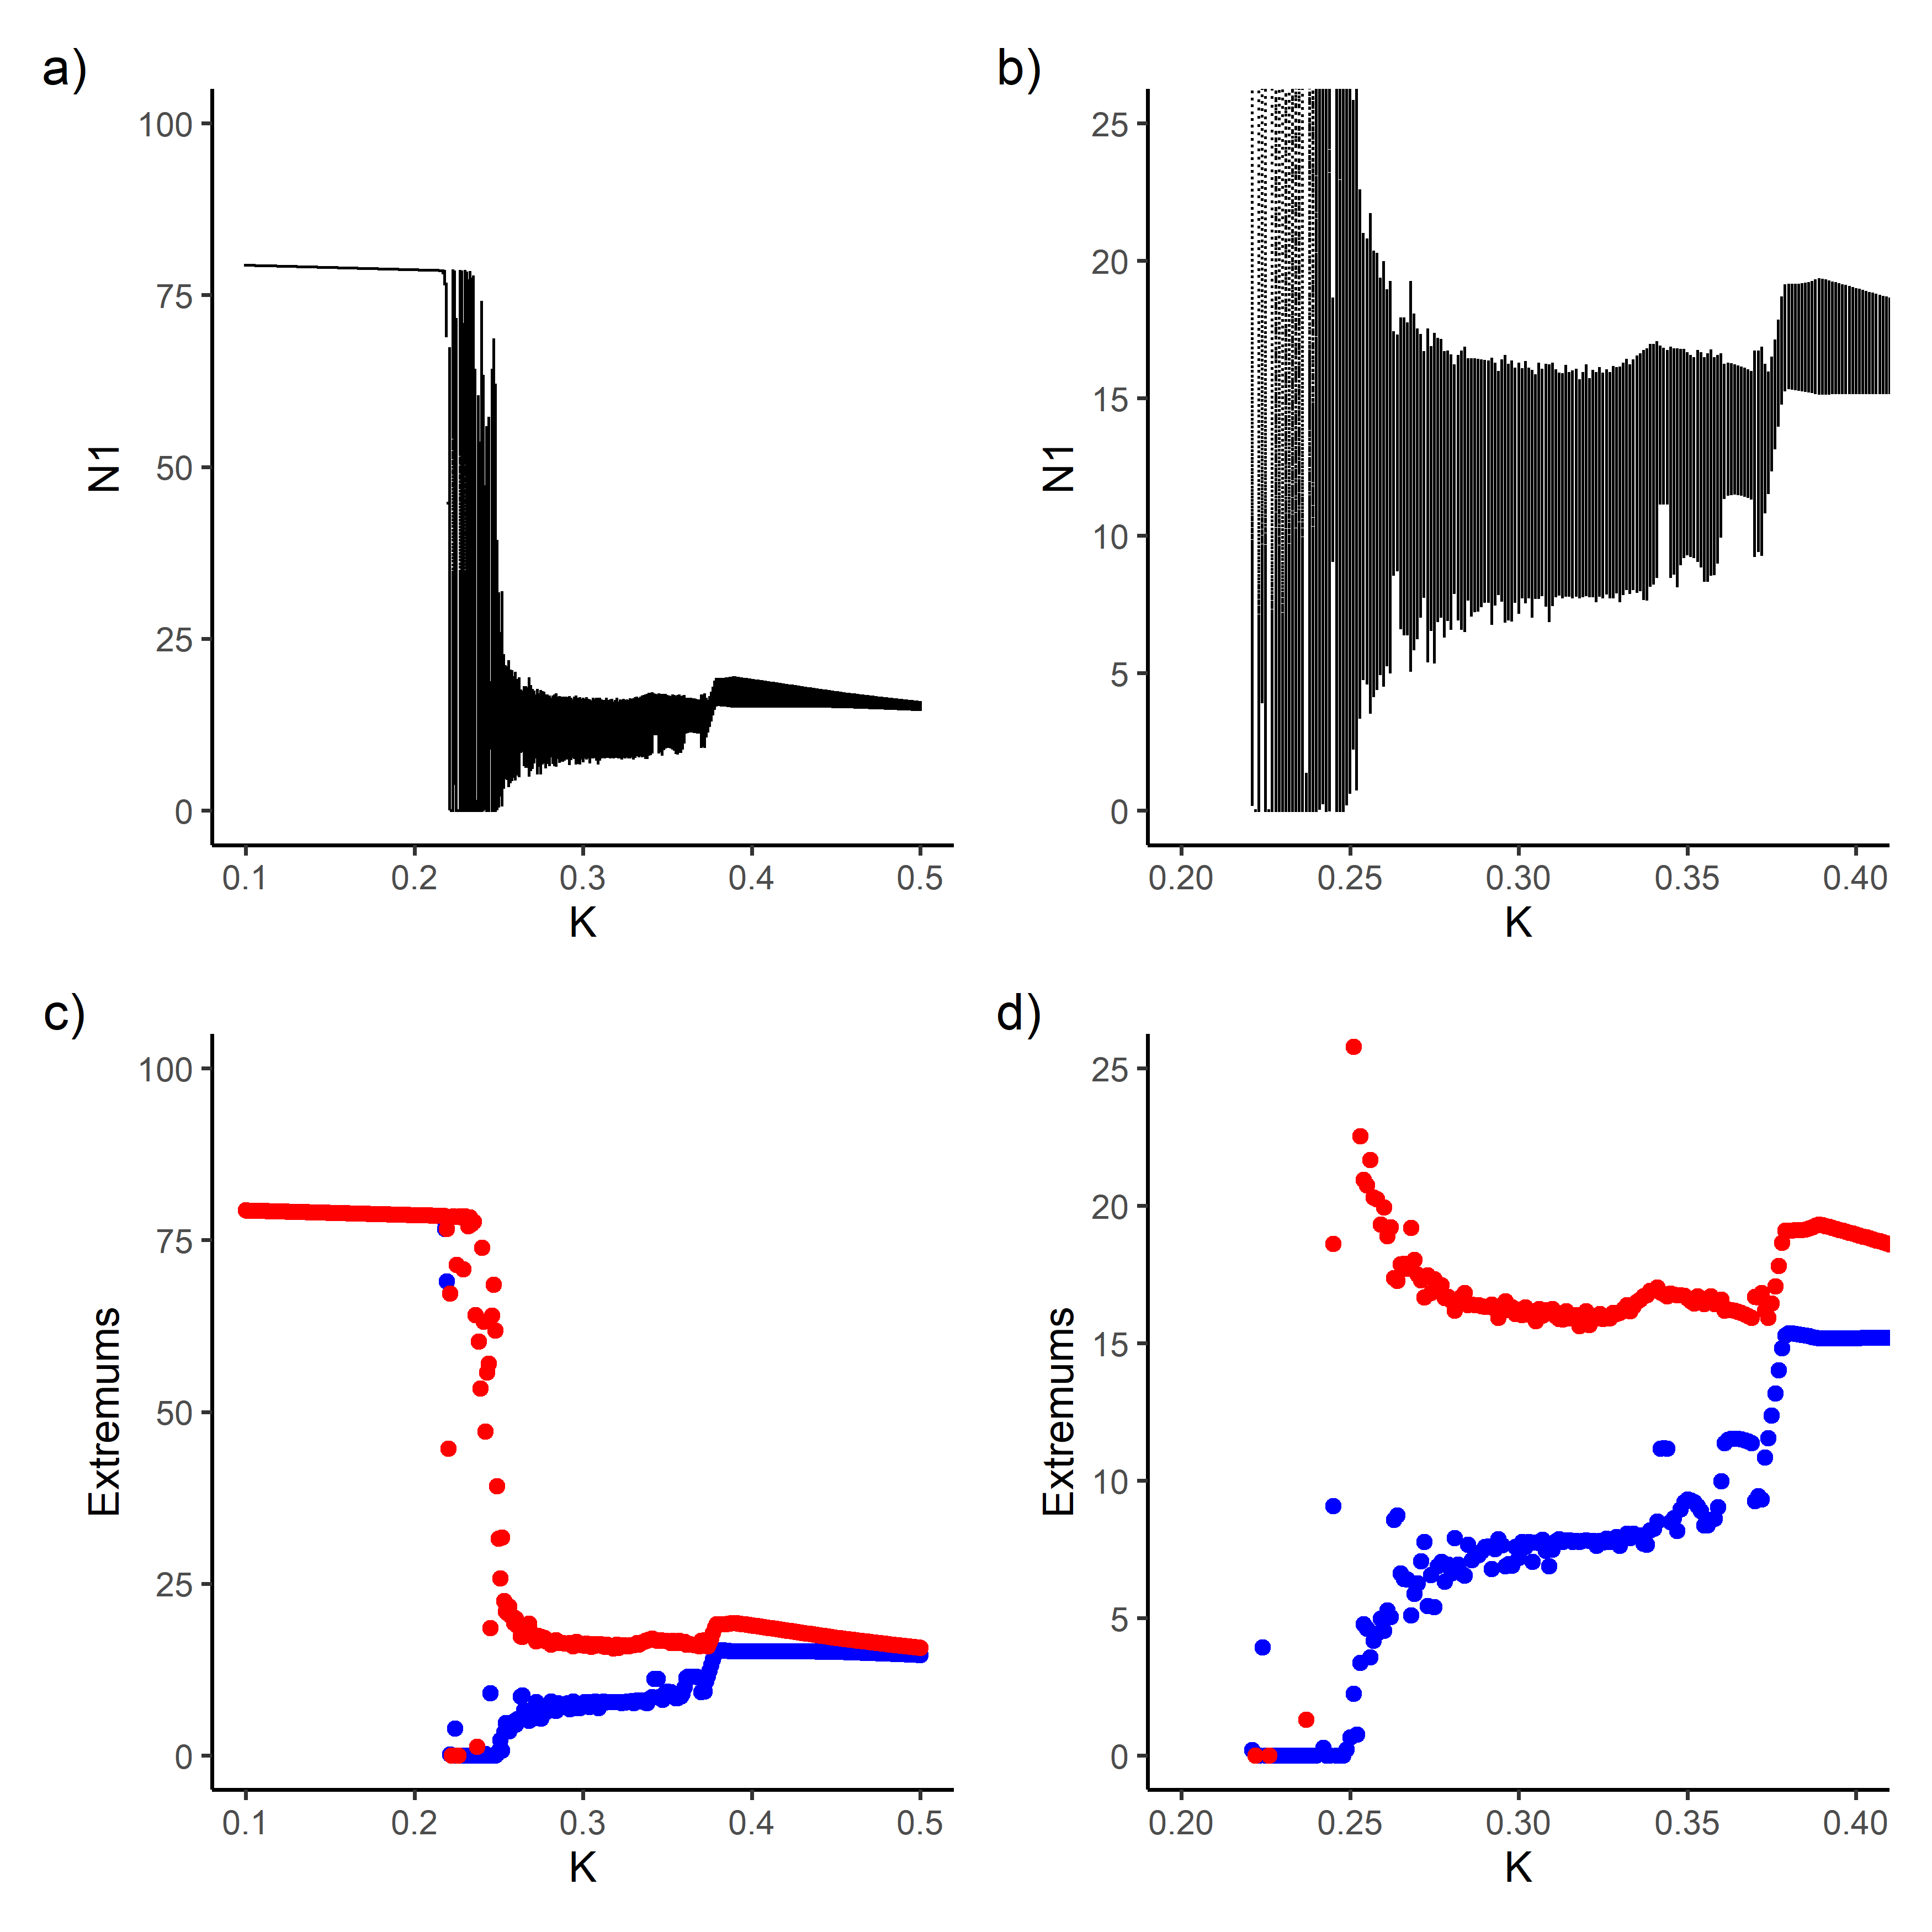
\includegraphics[width=1\textwidth]{../Code/Figures/Figure_3.png}
  \caption{Bifurcation diagram, for five species competing for five resources. a) All of the values of species 1, plotted during the period from $t=2,000$ to $t=4,000$ days, as a function of the half-saturation constant $K_{41}$. Part of a) is magnified in b). c) show the local minima and maxima of species 1, plotted during the period from t= 2,000 to t=4,000 days, as a function of the half-saturation constant $K_{41}$. Part of c) is magnified in d).}
  \label{figures:Fig3}
\end{center}
\end{figure}

The bifurcation diagram \ref{figures:Fig3} caption did not seem to correspond to the actual Figure, which seemed to display all of the points of the simulation between $t=2,000$ and $t=4,000$ rather that only the local extrema as the legend of the original article suggested. We have therefore chosen to draw those two options. 

\begin{figure}[H]
	\begin{center} 
		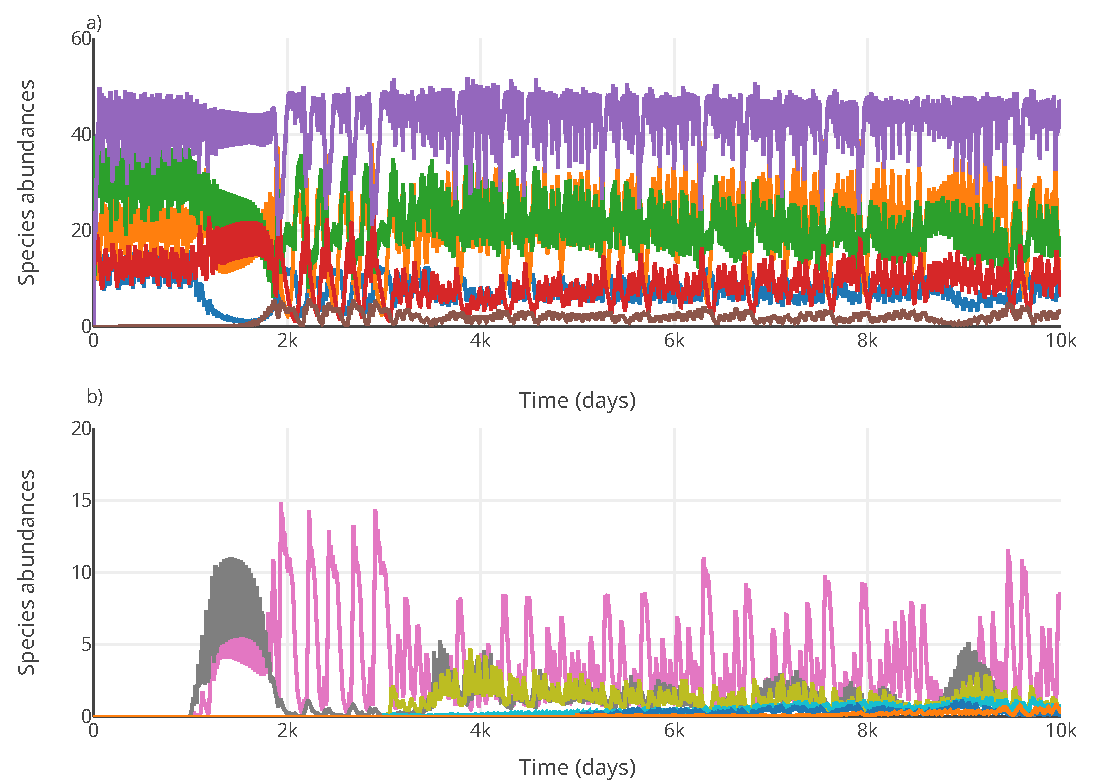
\includegraphics[width=0.86\textwidth]{../Code/Figures/Figure_4.pdf}
 		\caption{Competitive chaos and the coexistence of twelve species on five resources. a) abundances of species 1-6, b) abundances of species 7-12. }
 		\label{figures:Fig4}
	\end{center}
\end{figure}

\subsection{Numerical experiments}

For the first numerical experiment, which introduces species sequentially as in the original simulation, the distribution of the number of extant species is diplayed in Figure~\ref{figures:Figexp1bar}.

\begin{figure}[H]
	\begin{center} 
		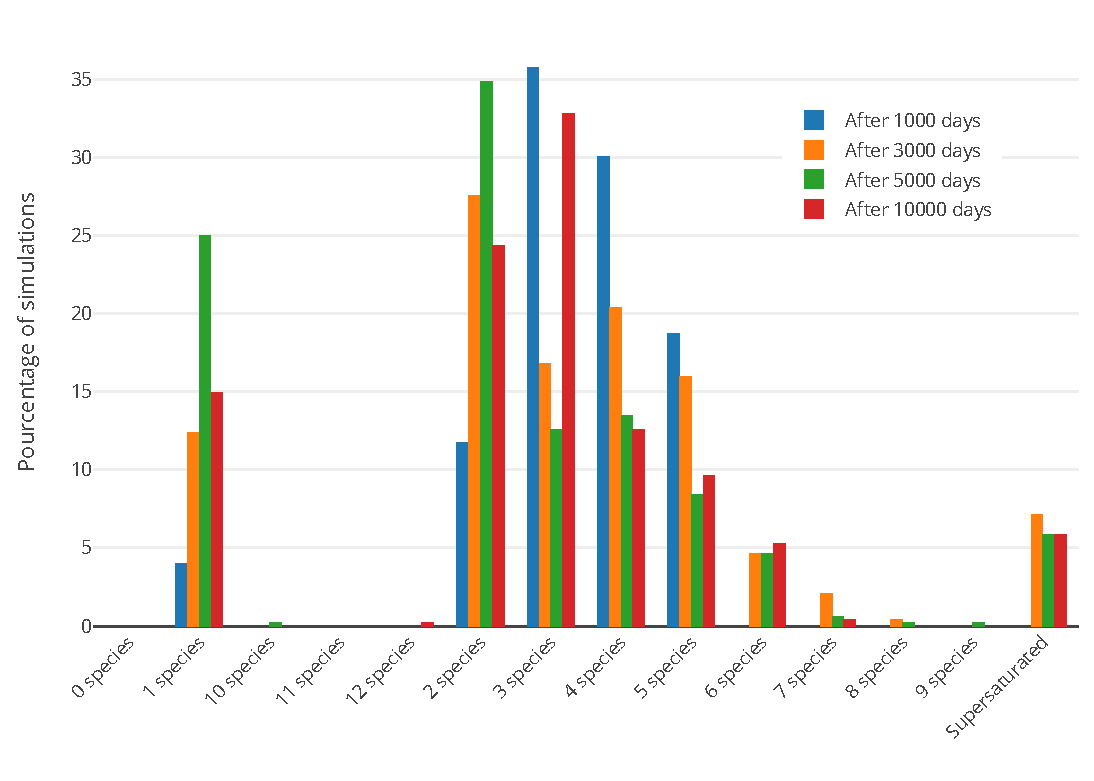
\includegraphics[width=0.86\textwidth]{../Code/Figures/Figure_exp1_bar.pdf}
 		\caption{Percentages of simulations with $x$ species present, or with observable supersaturated coexistence, at different times of the simulation for the first experiment. 500 simulations have been run in total and a species has been considered present if $N_i > 0.001$.}
 		\label{figures:Figexp1bar}
	\end{center}
\end{figure}

These percentages show that the persistence of five species or more is very unlikely, and that supersaturated coexistence may be present in a limited domain of parameter space.\\
\\
Community dynamics for the first experiment, with possible extinctions, are shown by Figure \ref{figures:Figexp1}. Note that panel 1 represents the original simulation with $r_i=1 ~\forall i$, while $r_i$ randomly varies between species for all other panels. 

\begin{figure}[H]
\begin{center} 
 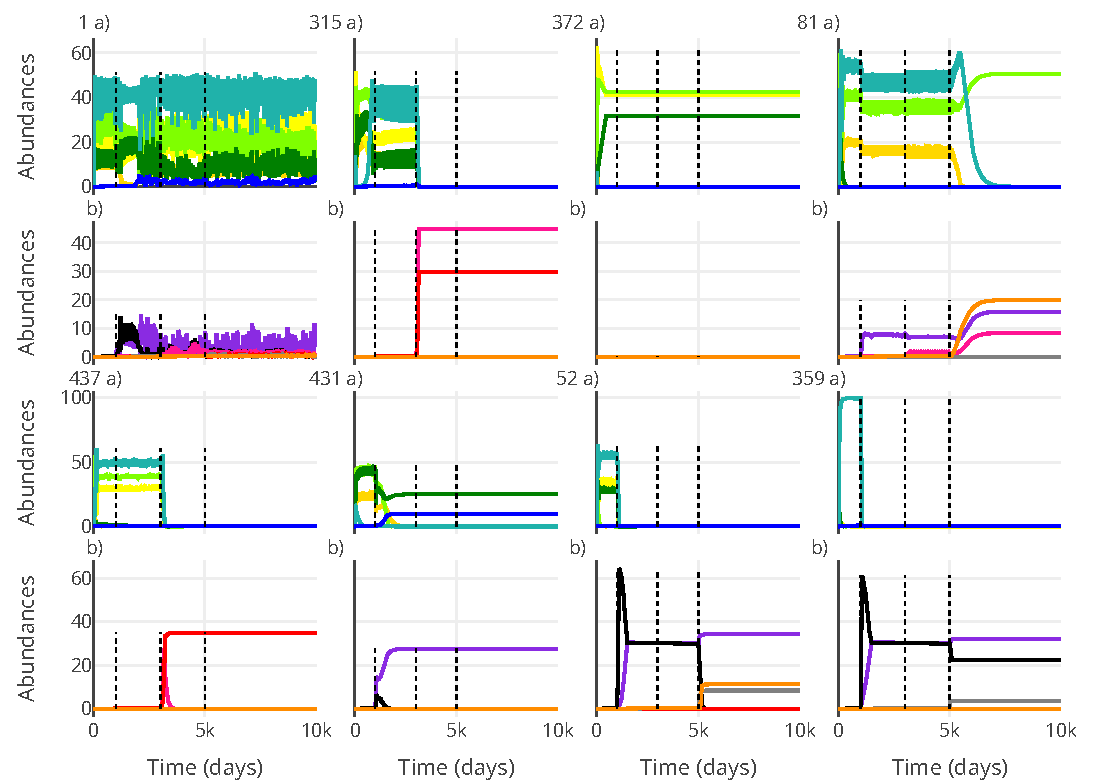
\includegraphics[width=1\textwidth]{../Code/Figures/Figure_exp1.pdf}
  \caption{Visualisation of eight different simulations of competitive chaos and coexistence of twelve species on five resources. It is identical to Figure 4 except that intrinsic growth rates $r_i$ are randomly varied. Except for the first panel, the simulations chosen were randomly picked among the 500 constituting the numerical experiment. Each couple of subplots is labelled with the number of the corresponding simulation. a) abundances of species 1-6, b) abundances of species 7-12. Dashed vertical lines represent the introduction of new species.}
  \label{figures:Figexp1}
\end{center}
\end{figure}

We observe contrasted stationary endpoints, possibly with some oscillations or chaos during the invasion process. As shown in Figure \ref{figures:Figexp1}, however, most species do not persist. 
%In many scenarios, at least a few species oscillated around stable points until additional species were introduced but sometimes these stable oscillations were never established in the first place.\\
%FB 30/06/2023: I have commented out this sentence because I do not understand what it means: if a fixed point is stable then there can be transient oscilations, but there cannot be stable oscillations (if the oscillations, i.e., the limit cycle is stable then the fixed point is usually not). Be careful to be very precise. The previous sentence about five species on five resources was clearer. 

\\
For the second experiment, introducing all species at once, the percentage of experiments with $x$ species present at different times of the simulation is displayed in Figure \ref{figures:Figexp2bar}.\\

\begin{figure}[H]
	\begin{center} 
		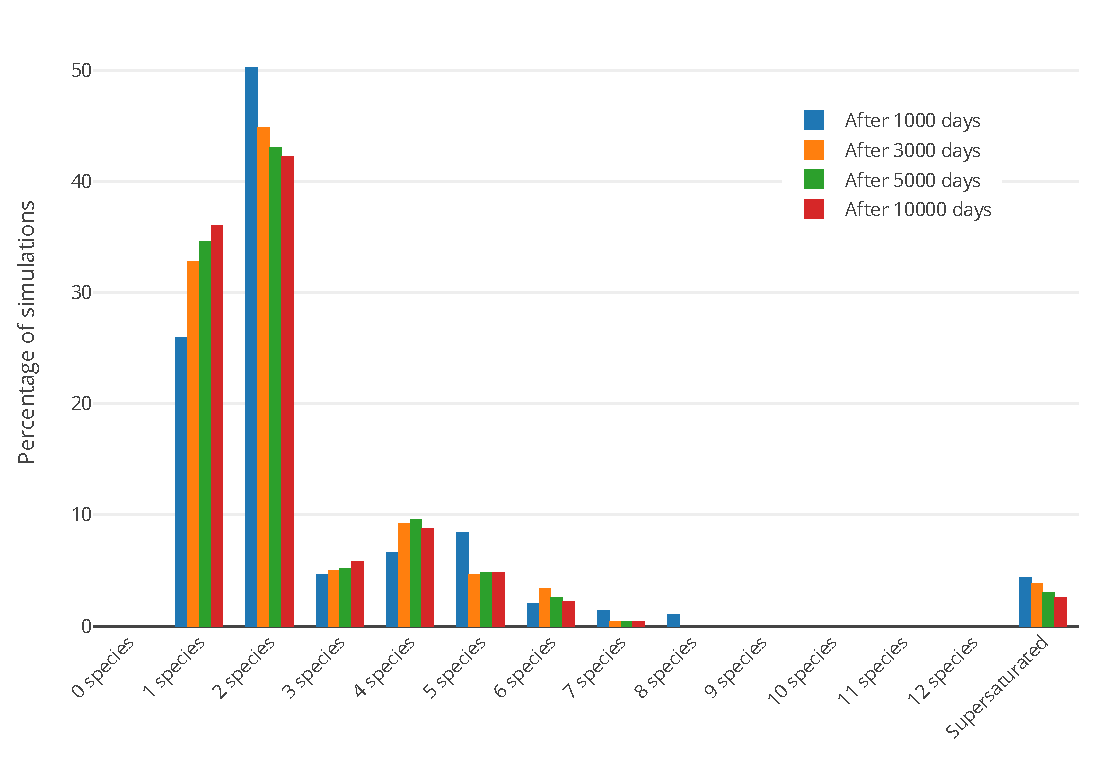
\includegraphics[width=0.86\textwidth]{../Code/Figures/Figure_exp2_bar.pdf}
 		\caption{Percentage of simulations with $x$ species present, or with observable supersaturated coexistence, at different times of the simulation for the second experiment. 500 simulations have been run in total and a species has been considered present if $N_i > 0.001$.}
 		\label{figures:Figexp2bar}
	\end{center}
\end{figure}

As before, a species has been considered present if $N_i > 0.001$ at the end of the simulation. The second experiment shows that persistence of five species or more is very unlikely when introducing all species at once (even more so than when introducing species sequentially), and that supersaturated coexistence is consequently very rare in this configuration.\\
\\
Community dynamics for the second experiment, with possible extinctions, are described in the following Figure \ref{figures:Figexp2}. Note that the subfigure 1 represents the original results with $r_i=1 ~\forall i$, while $r_i$ randomly varies as described in the methods for all other panels.

\begin{figure}[H]
\begin{center} 
 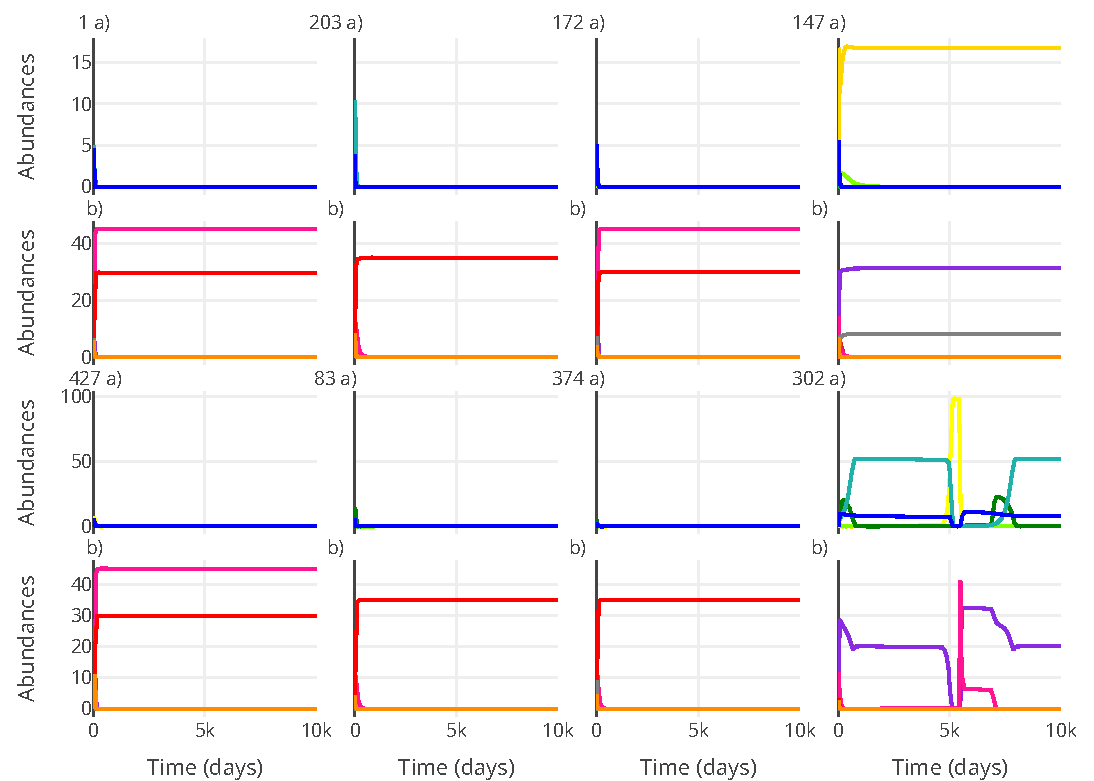
\includegraphics[width=1\textwidth]{../Code/Figures/Figure_exp2.pdf}
  \caption{Visualisation of eight different simulations of competitive chaos and coexistence of twelve species on five resources, following the Figure 4 method except that $r_i$ was randomly drawn for each of the species and all species were introduced at once. Except for the first panel (original parameters), the simulations illustrated were randomly picked among the 500 of the numerical experiment. Each couple of subplots is labelled with the number of the corresponding simulation. a) abundances of species 1-6, b) abundances of species 7-12.}
  \label{figures:Figexp2}
\end{center}
\end{figure}

As for the first experiment we mostly observed either fixed (non-oscillatory) stationary endpoints or oscillations, but with even less persistent species in the latter case, as shown in Figure \ref{figures:Figexp2}. %% FB 30/06/2023: Fig. 8 does not show that very well now, I think. 

\section{Discussion}

We were able to successfully replicate the figures of the original paper. There are minor differences in species dynamics in Figure~\ref{figures:Fig4}, which are arguably due to differences in numerical integration.\\

The additional numerical experiments showed that slightly changing the values of the $r_i$ parameters within a realistic range of values \cite{2015:Edwards} almost always prevents the coexistence of twelve species on five resources and mostly prevents supersaturated coexistence in general. This is true when introducing species sequentially as in the original paper, as well as all at once.\\

Our results corroborate those of Schippers et al. \cite{2001:Schippers}, who showed that supersaturated coexistence through chaos or oscillations requires particular sets of parameters values, which are not robust to small perturbations. Our results, using a slightly different kind of perturbation, are therefore consistent with their conclusion that supersaturated coexistence is unlikely to solve the paradox of the plankton. Additionally, there are other reasons (mixing, spatial structure) not considered here, which could render supersaturated coexistence unlikely \cite{2008:Roelke}. 
\newpage
\section{Appendix}

We present below additional time series for random parameter sets and for the two numerical experiments. This is meant to help the reader to gain a better view of the dynamical behaviors for these two numerical experiments. The legends are identical to those of Figures \ref{figures:Figexp1} and \ref{figures:Figexp2}.\\

\foreach \n in {1,2,3}{
\begin{figure}[H]
\begin{center} 
 \includegraphics[width=1\textwidth]{../Code/Figures/Figure_exp1_app_\n.pdf}
  \caption{Visualisation of eight other different simulations of competitive chaos and coexistence of twelve species on five resources. It is identical to Figure \ref{figures:Fig4} except that intrinsic growth rates $r_i$ are randomly varied, and complements Figure \ref{figures:Figexp1}. The simulations chosen were randomly picked among the 500 constituting the first numerical experiment. Each couple of subplots is labelled with the number of the corresponding simulation. a) abundances of species 1-6, b) abundances of species 7-12. Dashed vertical lines represent the introduction of new species.}
  \label{figures:Figexp1_app_\n}
\end{center}
\end{figure}
}

\foreach \n in {1,2,3}{
\begin{figure}[H]
\begin{center} 
 \includegraphics[width=1\textwidth]{../Code/Figures/Figure_exp2_app_\n.pdf}
  \caption{Visualisation of eight other different simulations of competitive chaos and coexistence of twelve species on five resources, following Figure \ref{figures:Fig4}, except that $r_i$ are randomly drawn for each of the species, and all species were introduced at once (complements \ref{figures:Figexp2}). The simulations shown were randomly picked among the 500 of the numerical experiment. Each couple of subplots is labelled with the number of the corresponding simulation. a) abundances of species 1-6, b) abundances of species 7-12.}
  \label{figures:Figexp2_app_\n}
\end{center}
\end{figure}
}





